\documentclass[letterpaper,preprint]{aastex}
\usepackage{bm}
\usepackage{calc}
\usepackage{amssymb, amsmath}
\usepackage{hyperref}

\newcommand{\fig}{Figure}
\newcommand{\figref}[1]{\mbox{\fig~\ref{#1}}}

\begin{document}
\title{Bayesian multi-band source detection}
\author{Dustin Lang}
\date{\today}
\maketitle

\section{Multi-band detection}

We will use the graphical model shown in \figref{model}.  We have
measurements of the flux of a source from multiple bands $i$, $f_i$.
We wish to infer the ``total'' scalar flux $F$.  The true spectral
energy distribution (SED) of the source, $S$, is unknown and we wish
to marginalize over it.  $S$ is a vector with as many elements as
there are bands $i$.

While we have stated this as a problem of inferring flux, this is
exactly the same problem as source detection, since \emph{detection
  maps} used for source detection are in units of flux, and we
typically are asking whether the inferred flux distribution satisfies
a detection criterion; We typically ask that the signal-to-noise, or
mean relative to the standard deviation, is above a threshold.

\begin{figure}[h!]
\begin{center}
\includegraphics[width=0.5\textwidth]{pgm}
\end{center}
\caption{Our probabilistic graphical model for inferring source flux
  $F$ given spectral energy distribution (SED) $S$ and observed fluxes
  $f_i$.\label{model}}
\end{figure}

\newcommand{\setfi}{\{ f_i \}}
\newcommand{\dd}{\textrm{d}}

We want to infer
\begin{eqnarray}
  p(F | \setfi) &=& \int p(F, S | \setfi) \dd S \\
  &=& \int \frac{p(\setfi | F, S) p(F, S)}{p(\setfi)} \dd S \\
  &\propto& \int \prod_i p(f_i | F,S) \, p(F) p(S) \dd S
\end{eqnarray}
where we have assumed the flux estimates are independent.  Further, we
will assume they are Gaussian distributed with known variances
$\sigma_i^2$.  We will define $S_i$ so that the expected flux in band
$i$ is $F S_i$.  For simplicity in this document, we will assume that
the elements of $S$ sum to unity, but that of course need not be the
case.

With the assumption of the Gaussian distributions of $f_i$, we have
\begin{eqnarray}
  p(F | \setfi) &\propto& \int \prod_i \exp{\left( -\frac{(f_i - F S_i)^2}{2 \sigma_i^2} \right)} p(F) p(S) \dd S \\
  &\propto& \int \prod_i \exp{\left( -\frac{ \left( F - \frac{f_i}{S_i} \right)^2}{2 \frac{\sigma_i}{S_i}^2} \right)} p(F) p(S) \dd S \\
  &\propto& \int \exp{\left(- \frac{\left( \sum_i \frac{f_i S_i}{\sigma_i^2} - F \right)^2}%
    {\frac{2}{\sum_i \frac{S_i^2}{\sigma_i^2}}} \right)} p(F) p(S) \dd S
\end{eqnarray}
where we have folded the normalization of the exponential into the
proportionality, rescaled the exponential to be in units of $F$, and
then taken the product of the exponentials through the usual
inverse-variance weighting.

Clearly the likelihood for $F$ is a Gaussian, so we can write the
signal-to-noise of our constraint on $F$ as
\begin{eqnarray}
\textrm{SN}(F | \setfi) &=& \Large\int \sum_i \frac{f_i S_i}{\sigma_i^2} \sqrt{\sum_i \frac{S_i^2}{\sigma_i^2}} \,\, p(F) p(S) \dd S 
\end{eqnarray}

\subsection{Example}

Let us examine a simple 2-band example.  We will take $f_1 = 5$, $f_2
= 10$, with errors $\sigma_1 = \sigma_2 = 1$.  The distribution of $F$
as we vary $S$ is shown in \figref{example}.  When the SED $S$ matches
the flux ratio of the sources, the signal-to-noise of our constraint
on $F$ is maximized, and achieves the sum of the individual
measurements added in quadrature, as expected.  Extreme values of $S$,
which imply that all the flux appears in one of the bands, lead to
inferred distributions of $F$ that match those of the input
measurements.


\begin{figure}
\begin{center}
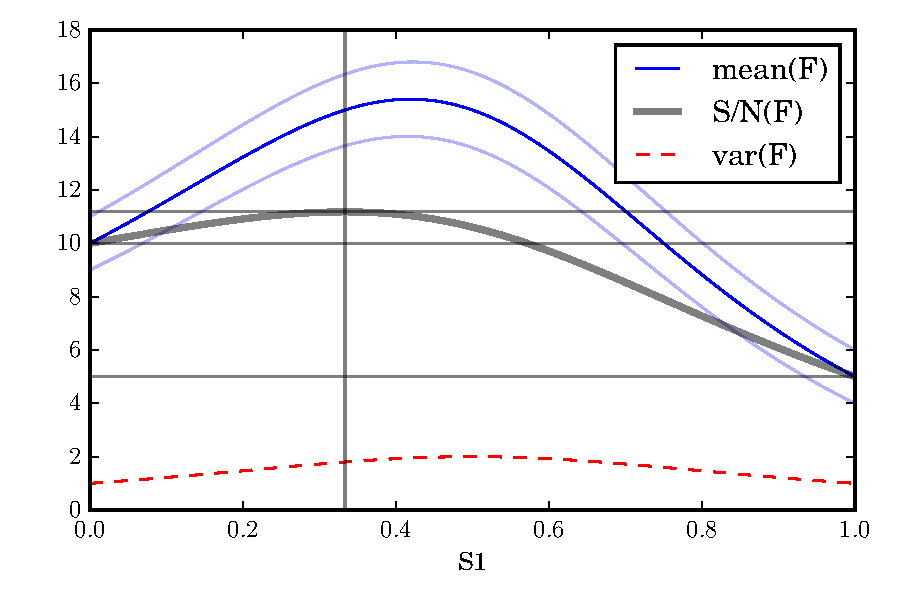
\includegraphics[width=0.8\textwidth]{bayes-00}
\end{center}
\caption{Example inferred flux distribution with respect to SED $S$
  for our example where $f_1 = 5$ and $f_2 = 10$, both with $\sigma_i
  = 1$.  When the SED $S_1 = 0$, this states that all the flux comes
  from the first band; the second band is irrelevant, so the inferred
  flux and signal-to-noise equals that of the measurement of $f_1$.
  Similarly, when the SED $S_1 = 1$, the mean and standard deviation
  match that of the second flux measurement $f_2 = 5 \pm 1$.  When
  $S_1$ matches the true ratio between $f_1$ and $f_2$, the flux
  estimate $F$ achieves maximum signal-to-noise, equal to the
  signal-to-noises of the measurements added in quadrature.
  \label{example}}
\end{figure}


\begin{figure}[p!]
\begin{center}
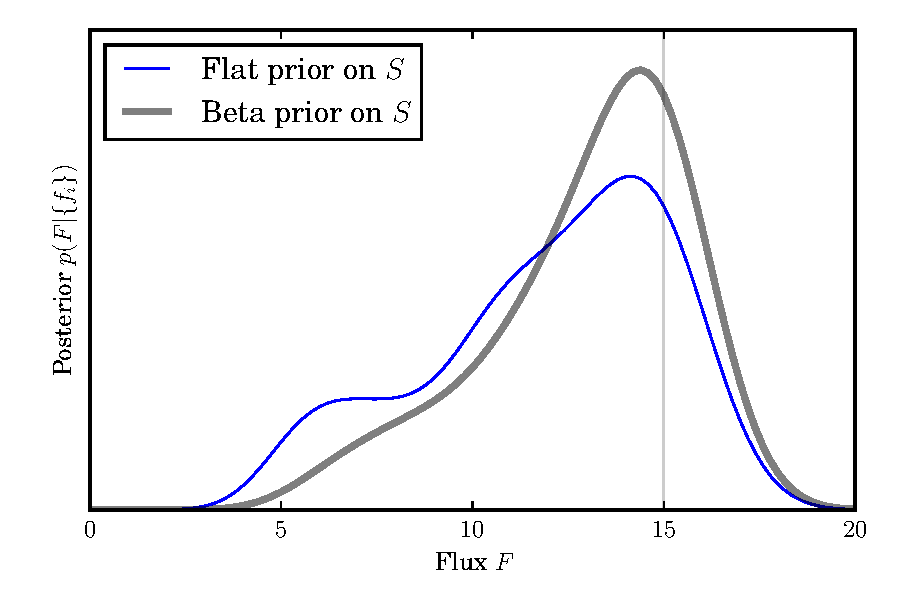
\includegraphics[width=0.7\textwidth]{bayes-01}
\end{center}
\caption{Posterior probability distributions of flux $F$ for our
  example, using an improper flat prior on $F$ and either a flat or
  beta distribution ($\alpha = \beta = 2$) for $S$.  The true total
  flux, $15$ is marked.
  \label{postflux}}
\end{figure}

\begin{figure}[p!]
\begin{center}
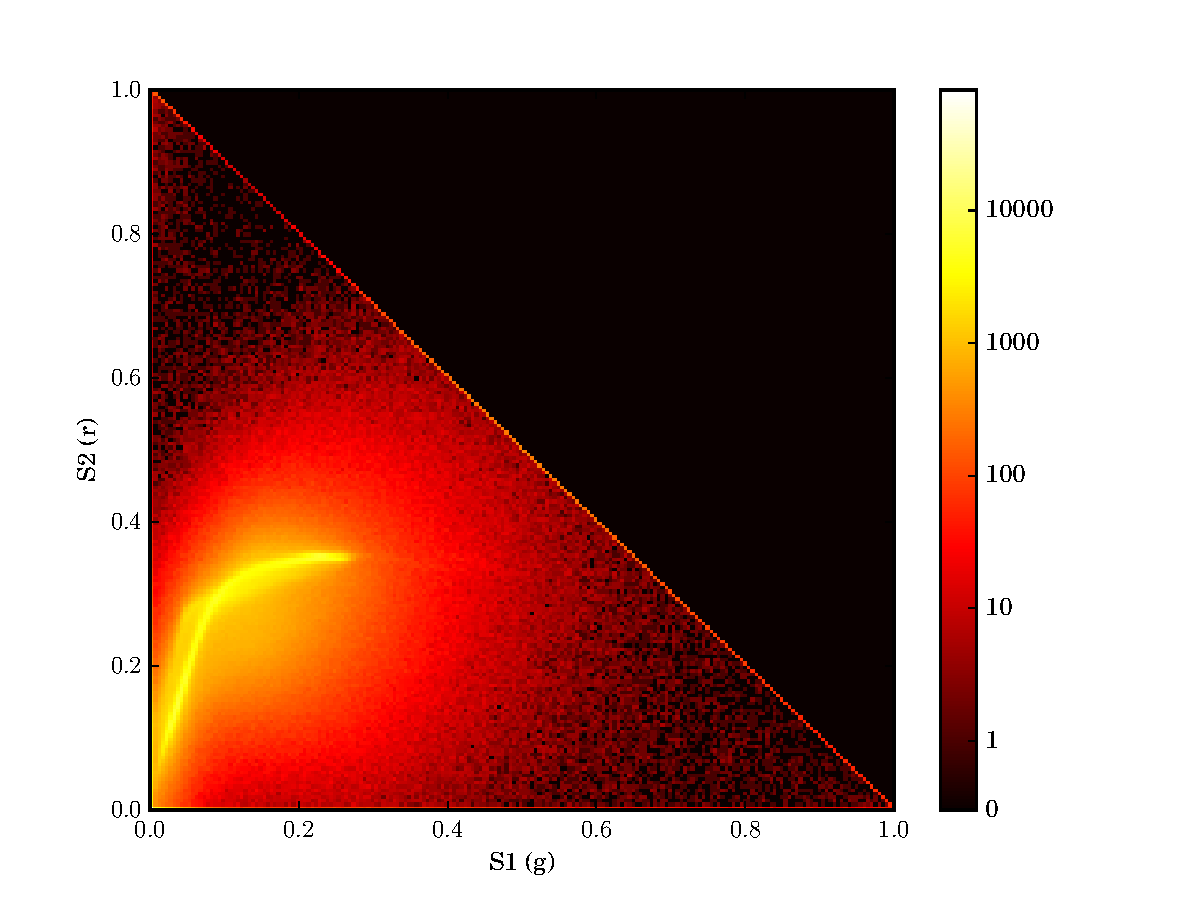
\includegraphics[width=0.8\textwidth]{bayes-05}
\end{center}
\caption{Where real astronomical sources live in SED space $S$.  This
  shows roughly 2 million sources from the DECam Legacy Survey
  measured in $g$, $r$, and $z$ bands.  The SED space is then the
  3-dimensional simplex, so a 2-dimensional plane embedded in 3-d.
  This is akin to a $grz - g$, $grz - r$ color space, where $grz$ is
  the sum of the fluxes in the three bands (ie, a broad filter).
  \label{Sgrz}}
\end{figure}



If we assign priors and marginalize over $S$, we can examine the
posterior distribution of $F$.  For $F$, let us for the moment use the
(improper) flat prior.  For $S$, we will use either a uniform prior,
or the beta prior (with parameters that place more probability in the
middle of the range; few sources emit in only one band).  Results for
these priors are shown in \figref{postflux}.


In practice, we will approximate the SED space $S$ with a small number
of weighted delta functions,
\begin{eqnarray}
p(S) &=& \frac{1}{\sum_i \alpha_i} \sum_i \alpha_i \delta_i(S(i))
\end{eqnarray}
where these should presumably be chosen based on the distribution of
real sources, with the number chosen to cover the space with
acceptable loss of signal-to-noise due to mismatches.

\figref{Sgrz} shows in this SED space the fluxes of sources measured
in the DECam Legacy Survey (DECaLS) Data Release 2, from $240 <
\textrm{RA} < 250$ and $5 < \textrm{Dec} < 10$, with fluxes measured
in $g$, $r$, and $z$ bands.  In astronomical parlance, this can be
seen as something like a $grz - g$, $grz - r$ color space.



\end{document}

